\documentclass[../main.tex]{subfiles}

\begin{document}
\section{Results}\label{sec:results}

Here we present figures showing the results of the simulations we have produced of the solar system. 

\subsection{Earth-Sun}

\begin{figure}
    \centering
    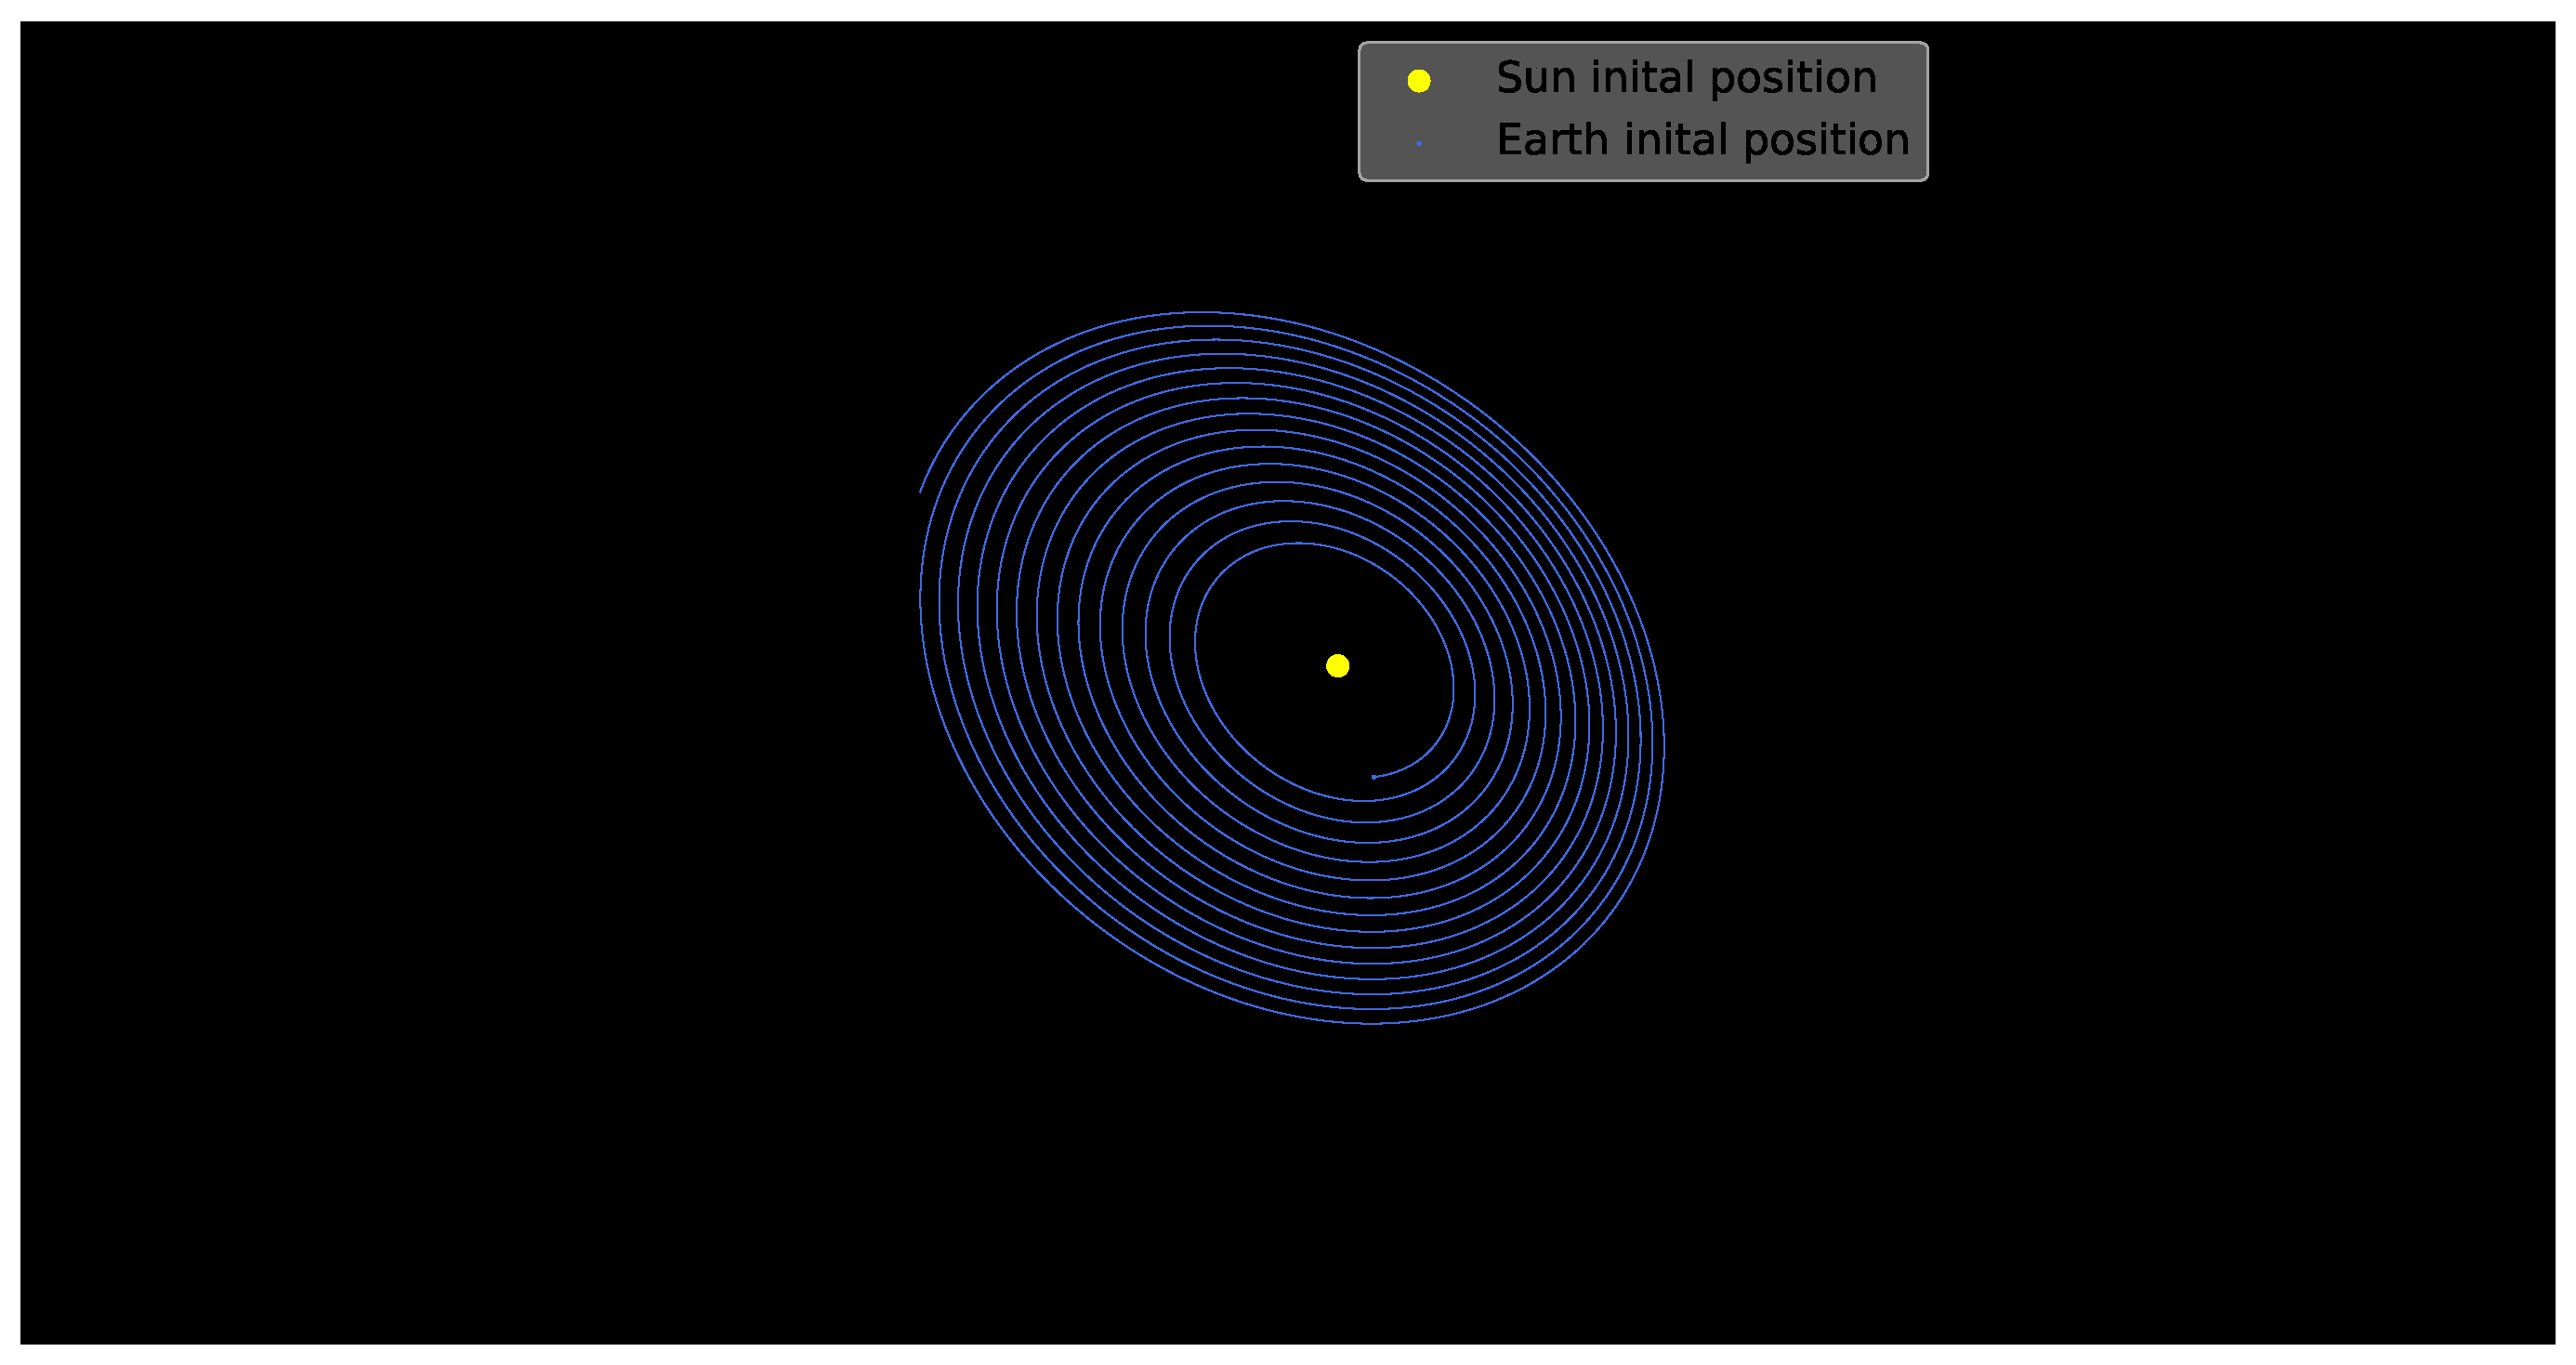
\includegraphics[trim=15cm 5.cm 11cm 0.cm, clip,width=0.8\textwidth]{../figures/Euler_Earth_Sun.pdf}
    \caption{Here is the Earth-Sun system simulated over 50 years using the Euler method. The Earth does not form a closed orbit, and is slowly escaping the gravitational well of the Sun. This is an error caused by the fact that the Euler method does not conserve energy.}
    \label{fig:earth-sun-euler}
\end{figure}

\subsection{Escape Velocity}

\begin{figure}
    \centering
    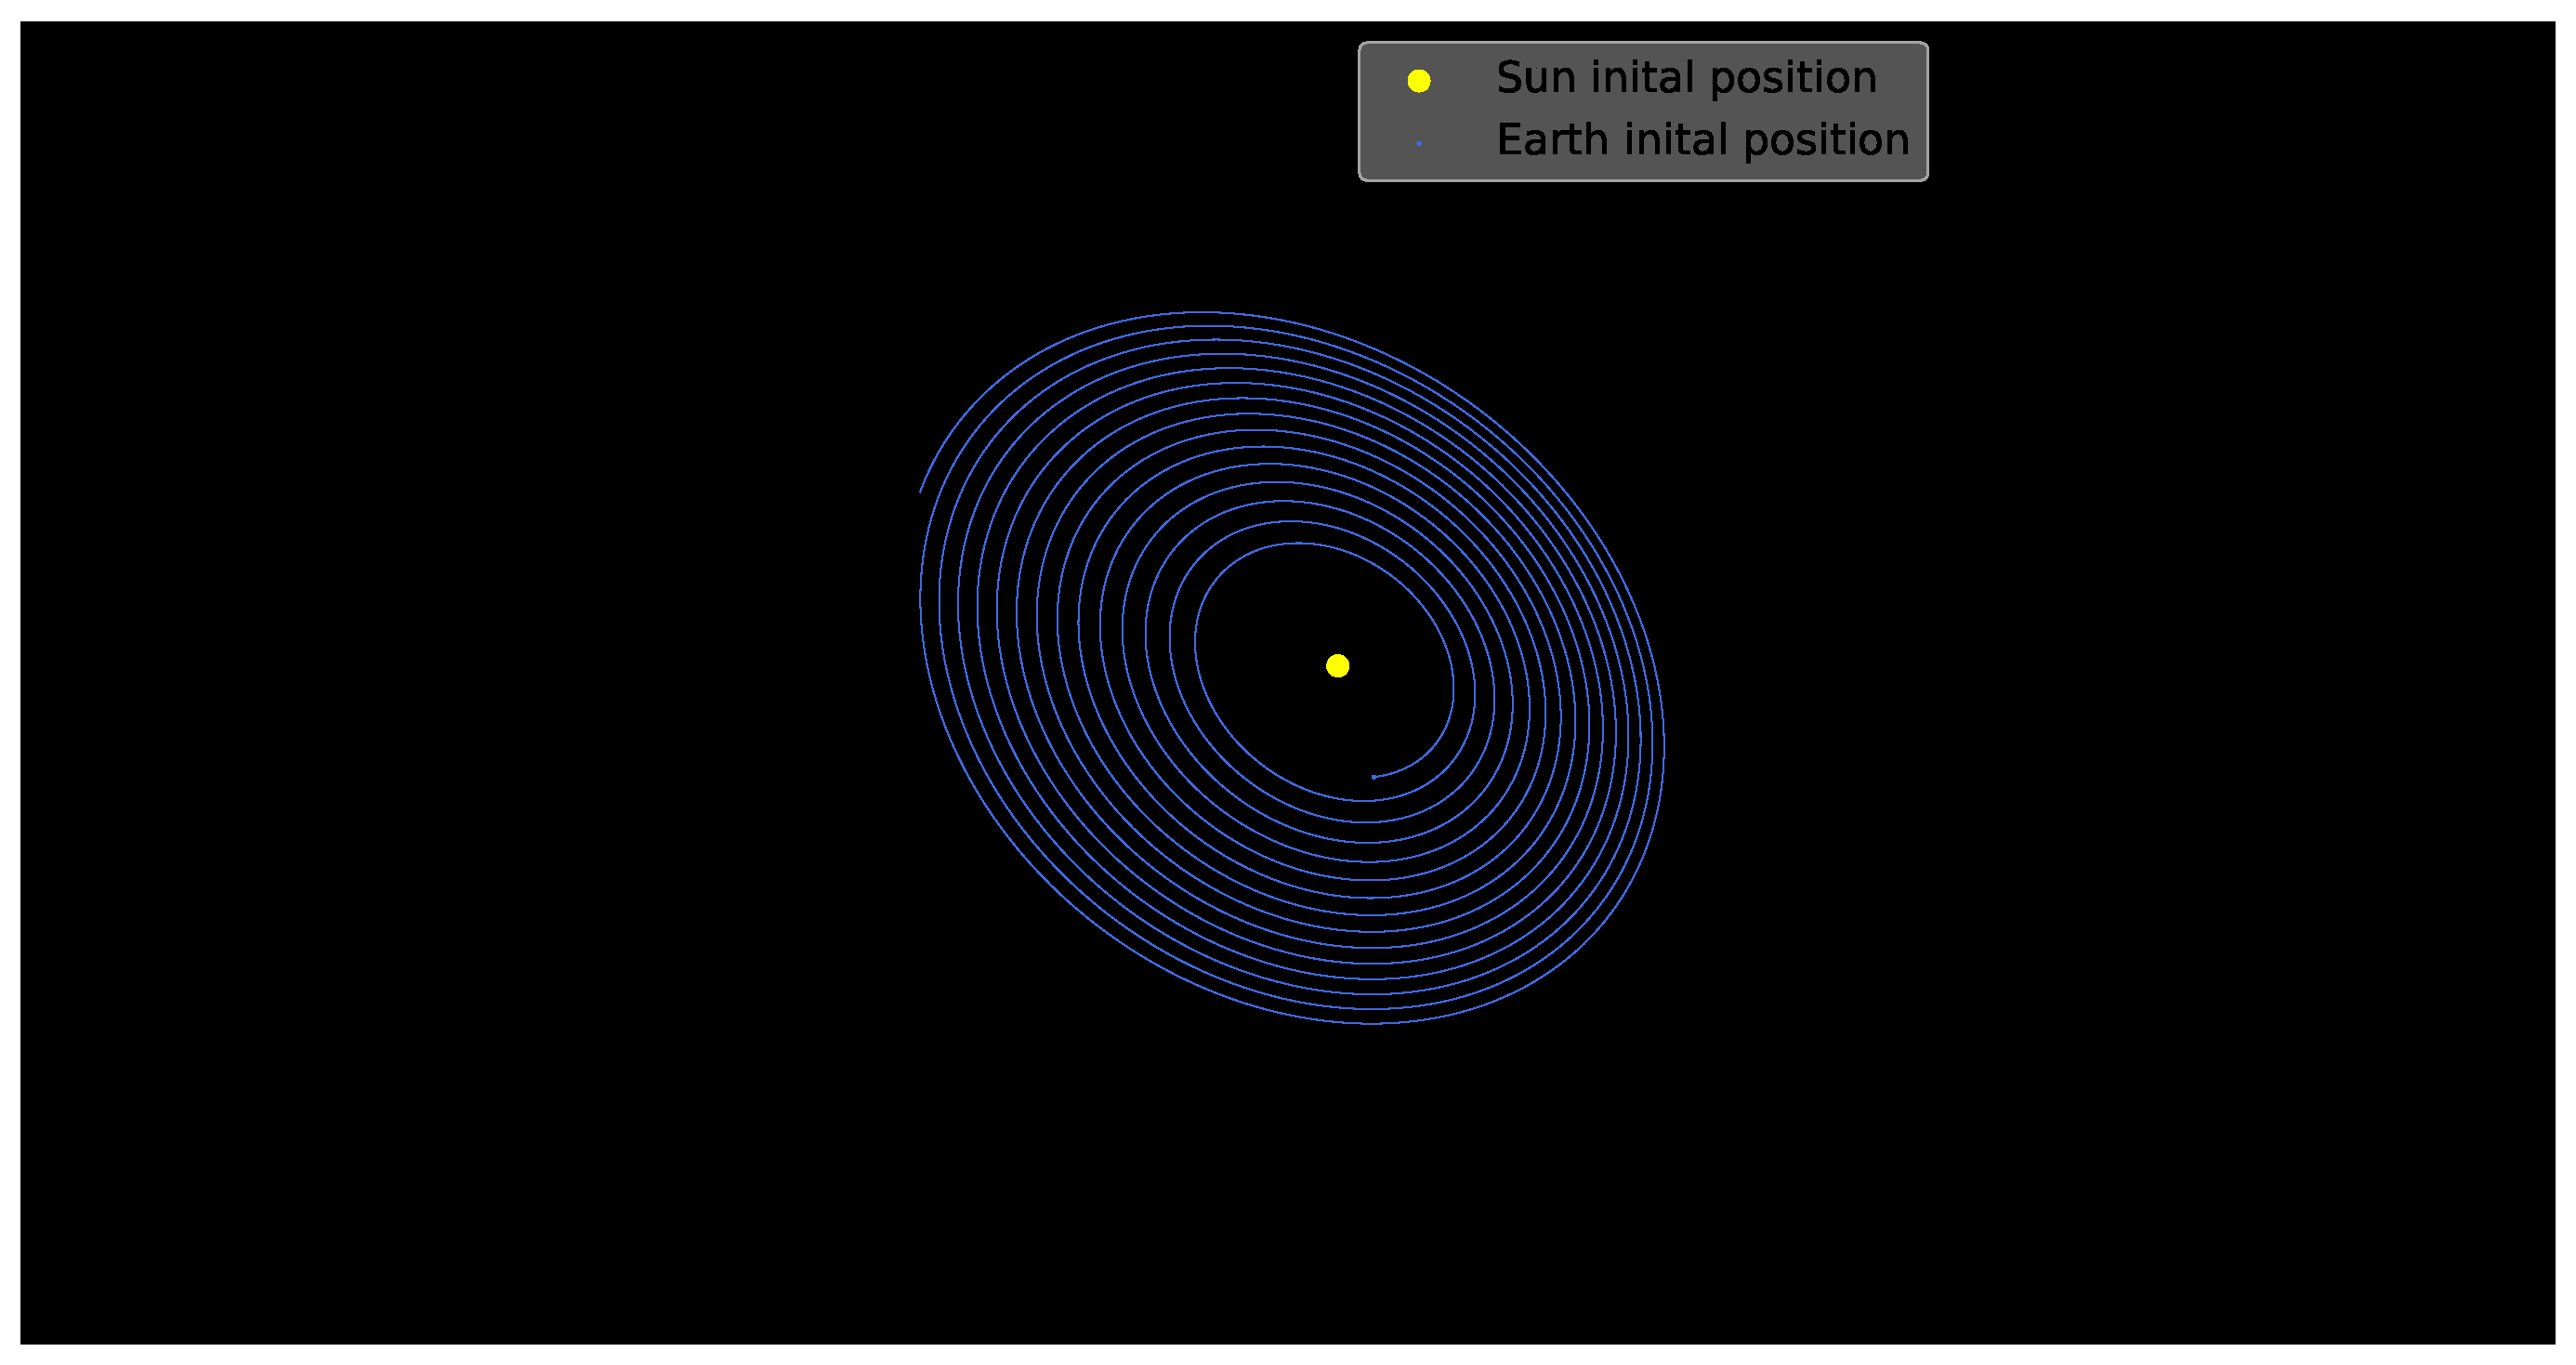
\includegraphics[trim=15cm 5.cm 11cm 0.cm, clip,width=0.8\textwidth]{../figures/Euler_Earth_Sun.pdf}
    \caption{Pictured is a simulation over 248 years, with the initial velocity of the earth set to $v_0 = 2.4296 \frac{\text{AU}}{\text{day}}$. By trial and error, this value seems to be enough for }
    \label{fig:my_label}
\end{figure}Figure of the Earth escaping the sun's gravitational field. Seems that the presence of the remaining planets does little to change the escape velocity. Preliminary results suggests that escape velocity is about 2.42E-02 AU/day, corresponding with the approximate 2.433E-02 AU/day analytic answer.

\subsection{Three-body Problem}

\subsection{Perihelion Precession}



\end{document}
